\chapter{The LHC and the CMS Detector}
\label{chap:cmsoverview}

Probing the \SM for signs of new physics would not be possible without the immensely complex electronics and machinery that makes the TeV energy scale accessible for the first time. This chapter will cover \CERN 's  Large Hadron Collider (\LHC) and the CMS detector, being the experiment the author is a member of. Section \ref{sec:cmsdetector} serves to introduce an overview of the different components of  the CMS detector, with more detail spent on those that are relevant in the search for Supersymmetric particles. Section \ref{sec:cmsobjects} will focus on event and object reconstruction again with more emphasis on jet level quantities which are most relevant to the author's analysis research. Finally Section \ref{sec:l1trigger} will cover work performed by the author, as service to the CMS Collaboration, in measuring the performance of the GCT component of the L1 trigger during the 2012-2013 run period.  


\section{The LHC}
\label{sec:thelhc} 

The \LHC is a storage ring, accelerator, and collider of circulating beams of protons or ions. Housed in the tunnel dug for the Large Electron-Positron collider (LEP), it is approximately 27 km in circumference, 100 m underground, and straddles the border between France and Switzerland outside of Geneva. It is currently the only collider in operation that is able to study physics at the TeV scale.  A double-ring circular synchrotron, it was
designed to collide both proton-proton (pp) and heavy ion (PbPb) with a centre of mass energy $\sqrt{s} = $ 14 \TeV at a final design luminosity of $10^{34}$cm$^{-2}$s$^{-1}$. \\

These counter-circulating beams of protons/Pb ions are merged in four sections around the ring to enable collisions of the beams, with each interaction point being home to one of the four major experiments; ALICE \cite{alicetdr} , ATLAS \cite{atlastdr}, CMS \cite{cmstdr} and LHCb \cite{lhcbtdr} which record the resultant collisions. The layout of the \LHC ring is shown in Figure \ref{fig:lhc-ring}. The remaining four sections contain acceleration,collimation and beam dump systems. In the eight arc sections, the beams are steered by magnetic fields of up to 8 \T provided by super conduction dipole magnets, which are maintained at temperatures of 2 \K using superfluid helium. Additional magnets for focusing and corrections are also present in straight sections within the arcs and near the interaction regions where the detectors are situated. \\


\begin{figure}[!h]

\centering
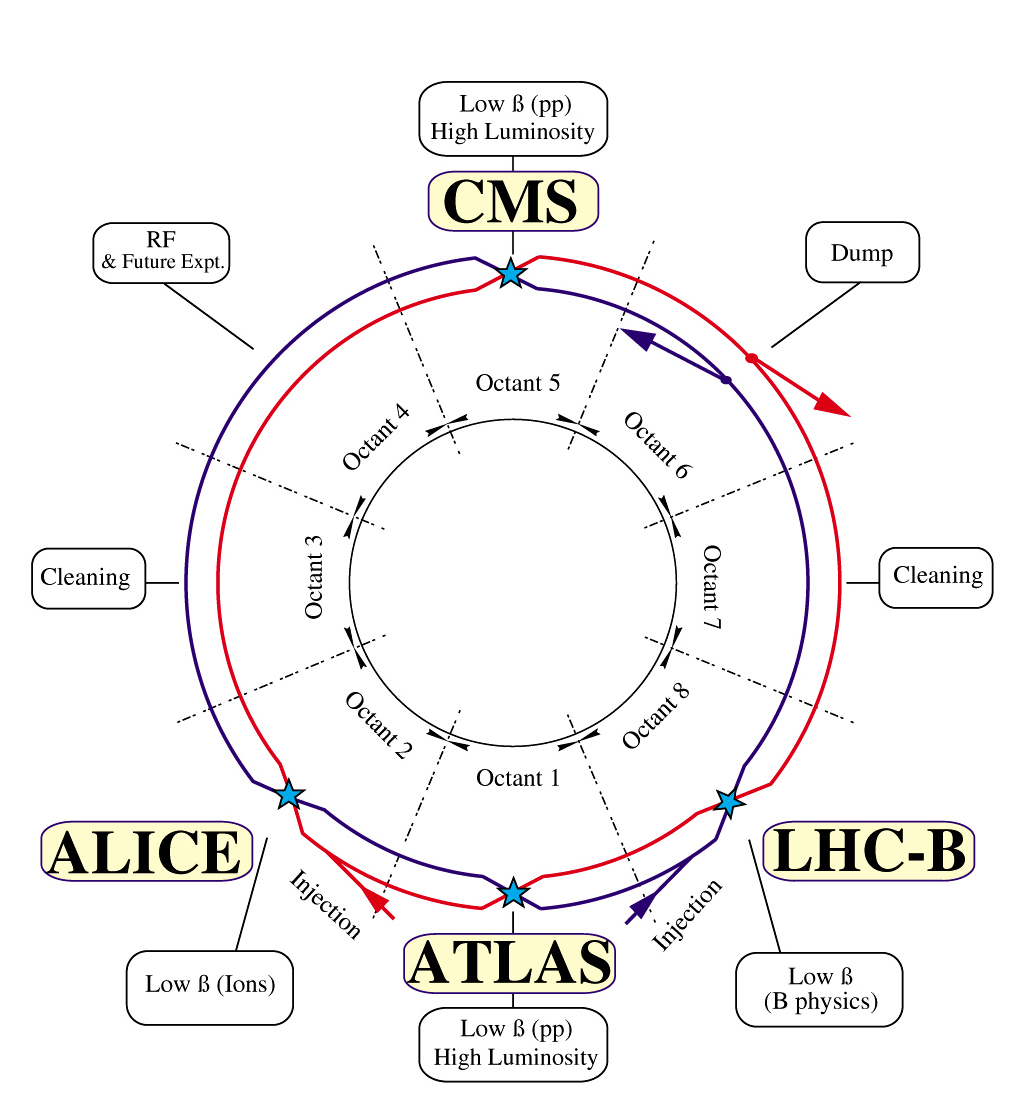
\includegraphics[width=0.65\textwidth]{plots/lhc-ring-photo.png}
\caption[A top down layout of the \LHC.]{A top down layout of the \LHC. \cite{Jean-Luc:841573}}  
\label{fig:lhc-ring}
\end{figure}


Proton beams are formed inside the Proton Synchrotron (PS) from bunches of protons 50 \ns apart with an energy of 26 \GeV. The protons are then accelerated in the Super Proton Synchrotron(SPS) to 450 \GeV  before being injected into the \LHC. These \LHC proton beams consists of many "bunches" i.e. approximately $1.1 \times 10^{11}$  protons localized into less than 1 \ns in the direction of motion. Before collision the beams are ramped to 4 \TeV (2012) per beam in a process involving increasing the current passing through the dipole magnets. Once the desired \com energy is reached then the beams are allowed to collide at the interaction points. The luminosity falls regularly as the run progresses as protons are lost in collisions, and eventually the beam is dumped before repeating the process again. \\

In the early phase of prolonged operation after the initial shutdown the machine operated in 2010-2011 at 3.5 \TeV per beam, \com $=$ 7 \TeV, delivering 6.13 \fb of data \cite{LHClumo}. During the 2012-2013 run period, data was collected at an increased \com $=$ 8 \TeV improving the sensitivity of searches for new physics. Over the whole run period 23.3 \fb of data was delivered of which 21.8 \fb was recorded by the \CMS detector \cite{LHClumo}. A total of 12 \fb of 8 \TeV certified data was collected by October 2012, and it is this data which forms the basis of the results discussed within this thesis.

\begin{figure}[!h]

\centering
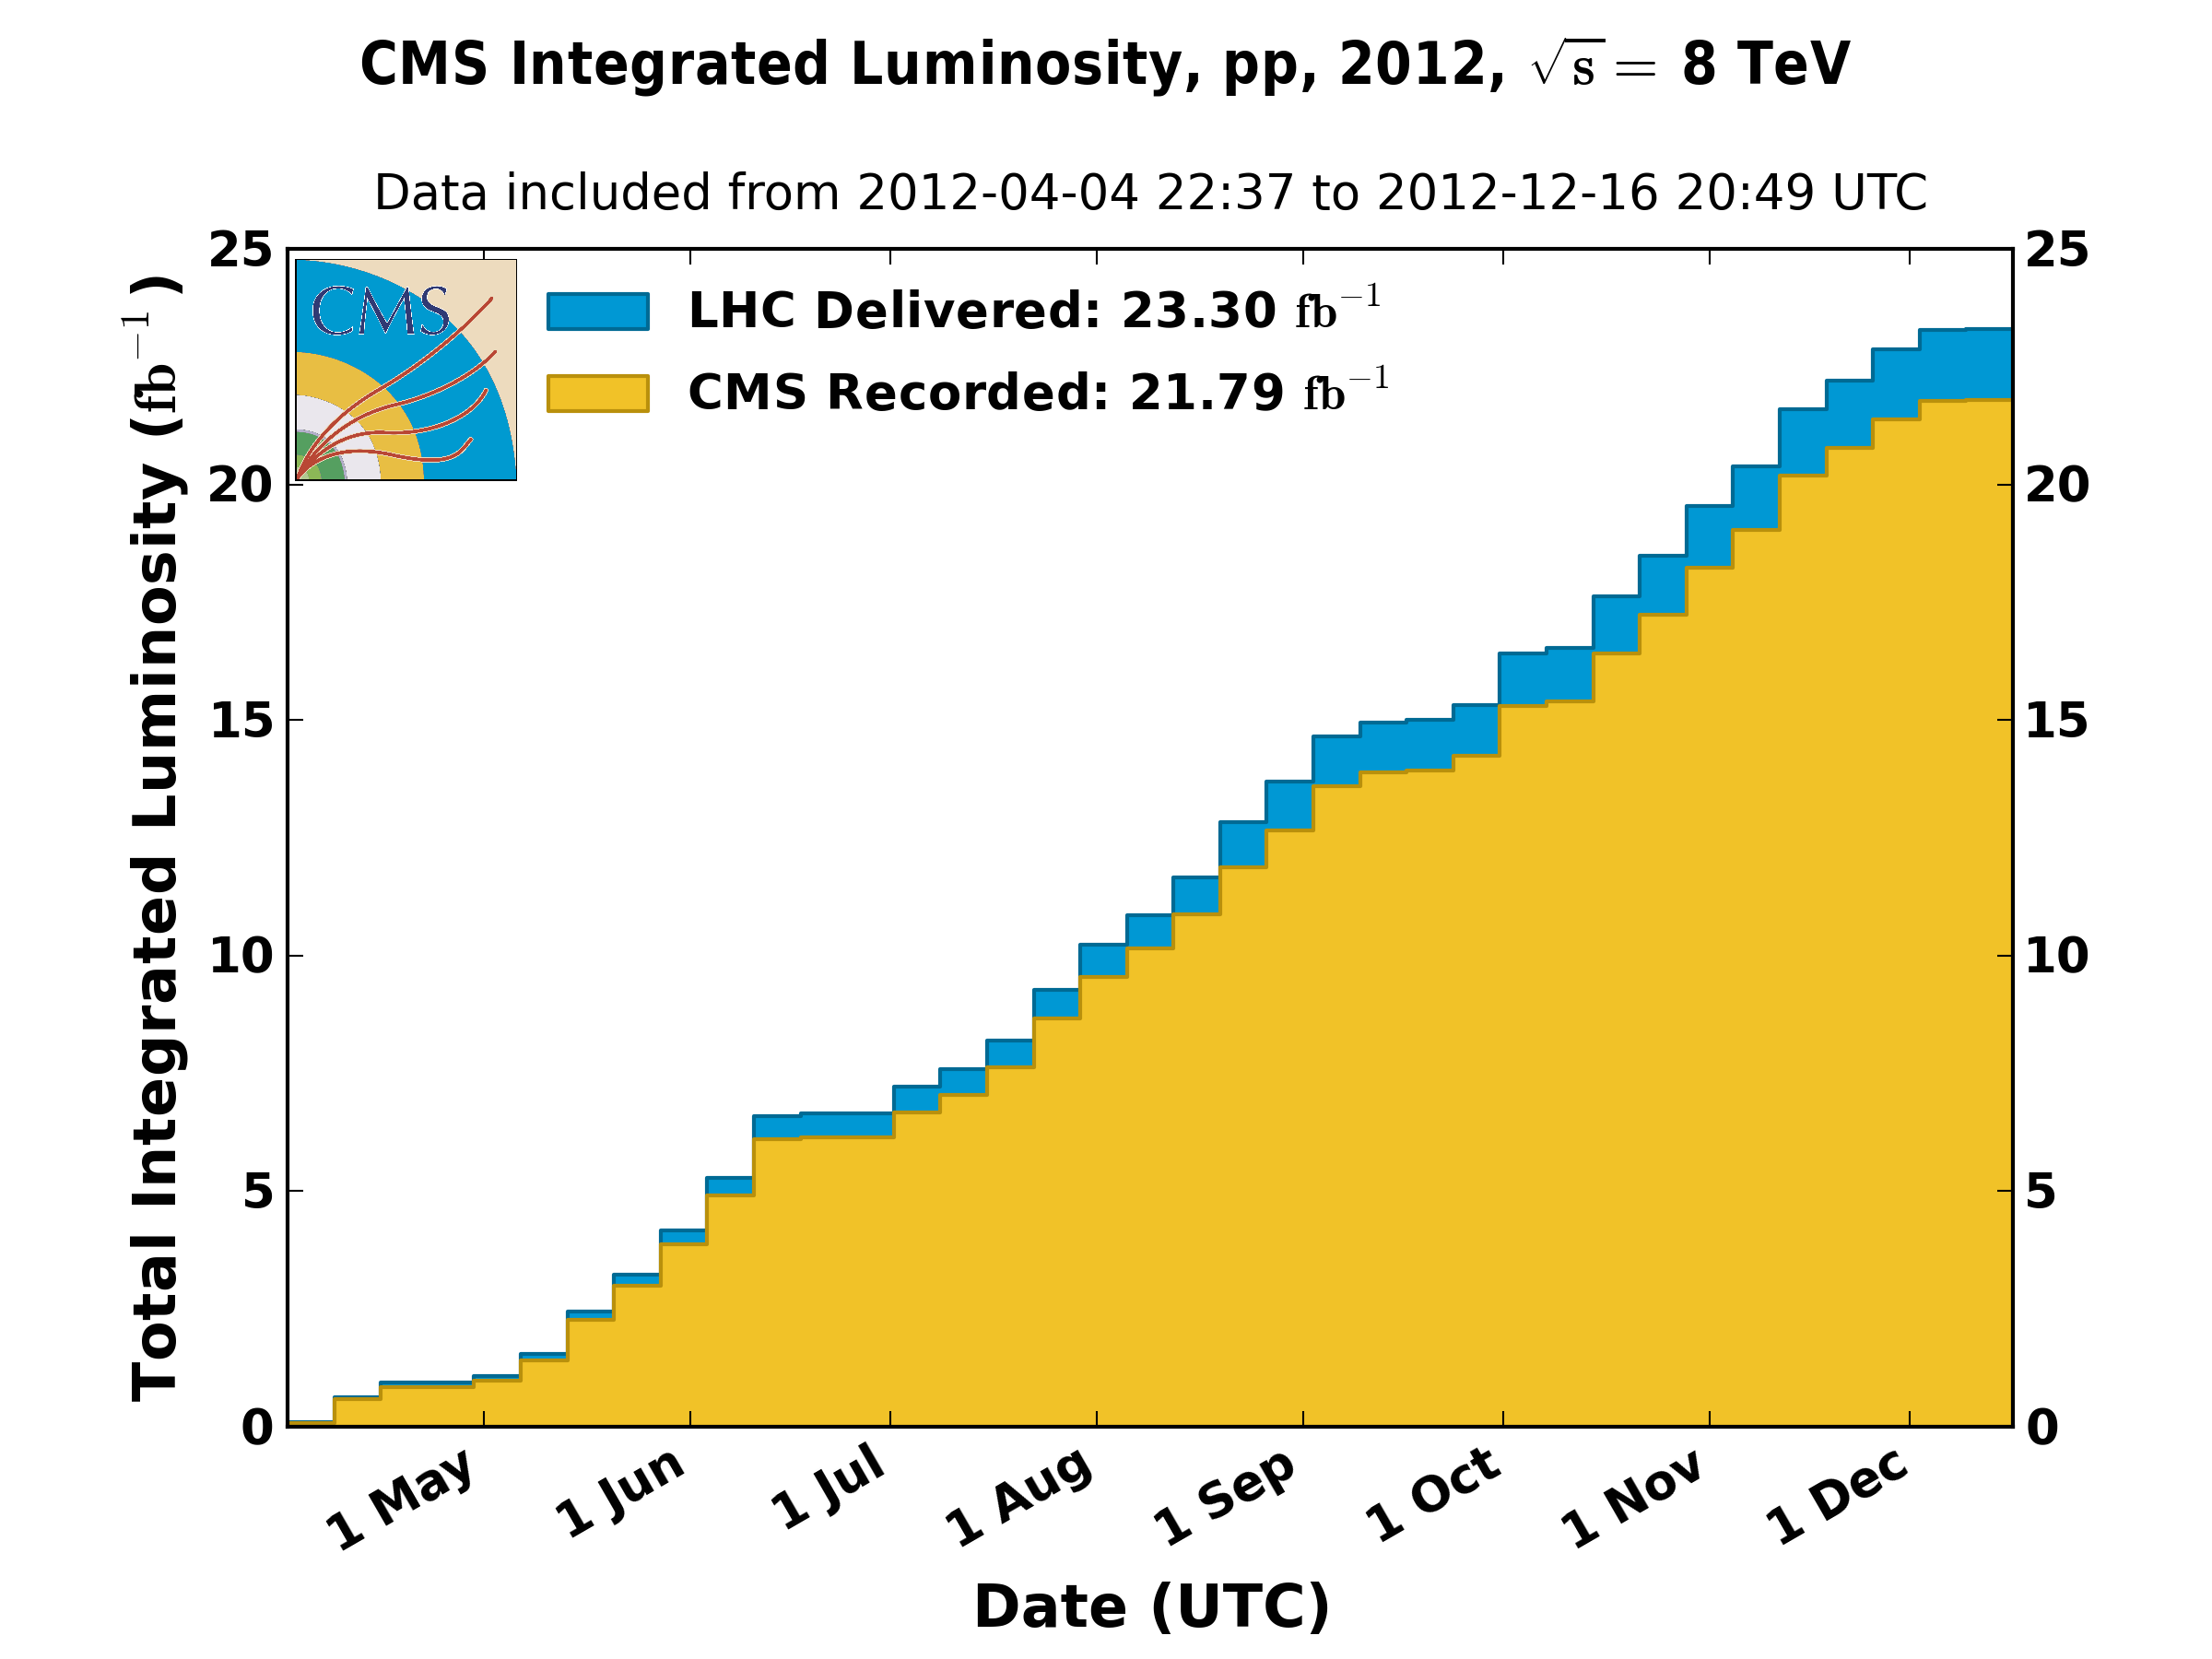
\includegraphics[width=0.65\textwidth]{plots/lhc-lumo-8tev.png}
\caption[The total integrated luminosity delivered to and collected by \CMS during the 2012 8 \TeV \pp runs]{The total integrated luminosity delivered to and collected by \CMS during the 2012 8 \TeV \pp runs.}  
\label{fig:lhc-ring}
\end{figure}


\section{CMS detector}
\label{sec:cmsdetector}

The Compact Muon Solenoid (\CMS) detector is one of two general purpose detectors at the \LHC designed to search for new physics. The detector is designed to provide efficient identification and measurement of many physics objects including photons, electrons, muons, taus, and hadronic showers over wide ranges of transverse momentum and direction. Its nearly 4$\pi$ coverage in solid angle allows for accurate measurement of global transverse momentum imbalance. These design factors give \CMS the ability to search for direct production of \SUSY particles at the \TeV scale, making the search for Supersymmetric particles one of the highest priorities among the wide range of physics programmes at \CMS.


\section{Object Definition}
\label{sec:cmsobjects}

Object stuff

\subsection{Jets}
\label{subsec:cmsobjects-jets}

Jets

\subsection{B-tagging}
\label{subsec:cmsobjects-btagging}

B-tagging

\section{L1 Trigger}
\label{sec:l1trigger}


L1 Work
